\subsection{Folgeregelung mit Störungsunterdrückung}
    Wenn man den LQRI-Ansatz um die feedforward Signale $u_\infty$ und $x_\infty$ erweitert, um auf eine Referenz mit Störungsunterdrückung zu regeln.
    
    Da nun auf eine Referenz geregelt wird, muss der Fehler im Zustand $ v(t)$ neu definiert werden: 
    \[v(t) = \int^t_0e(\tau)d\tau = \int^t_0(r(\tau)-y(\tau))d\tau\]
    Die Ableitung des Zustands lautet nun: 
    \begin{align*}
        \frac{d}{dt}\Tilde{x}(t) = \begin{bmatrix}A\cdot x(t) + B \cdot ( u(t) + w(t))\\r(t)-y(t)\end{bmatrix}\\
        = \underbrace{\begin{bmatrix}A&0\\-C & 0\end{bmatrix}}_{\Tilde{A}}\cdot\underbrace{\begin{bmatrix}x(t) \\v(t)\end{bmatrix}}_{\Tilde{B}}+\begin{bmatrix}B \\ 0 \end{bmatrix} \cdot(u(t)+w(t))+\begin{bmatrix}0 \\I\end{bmatrix}\cdot r(t).
    \end{align*}
    Die Lösung des Problems folgt:
    \begin{align*}
        \{\Tilde{A},\Tilde{B},\Tilde{Q},R\}\rightarrow \Tilde{K}=[\,K, - K_I]\, \in \mathbb{R}^{m\times(n+m)},\\
        u(t) = u_\infty-K\cdot(x(t)-x_\infty)+K_I\cdot v(t).
    \end{align*}
    
    \begin{figure}[H]
        \centering
        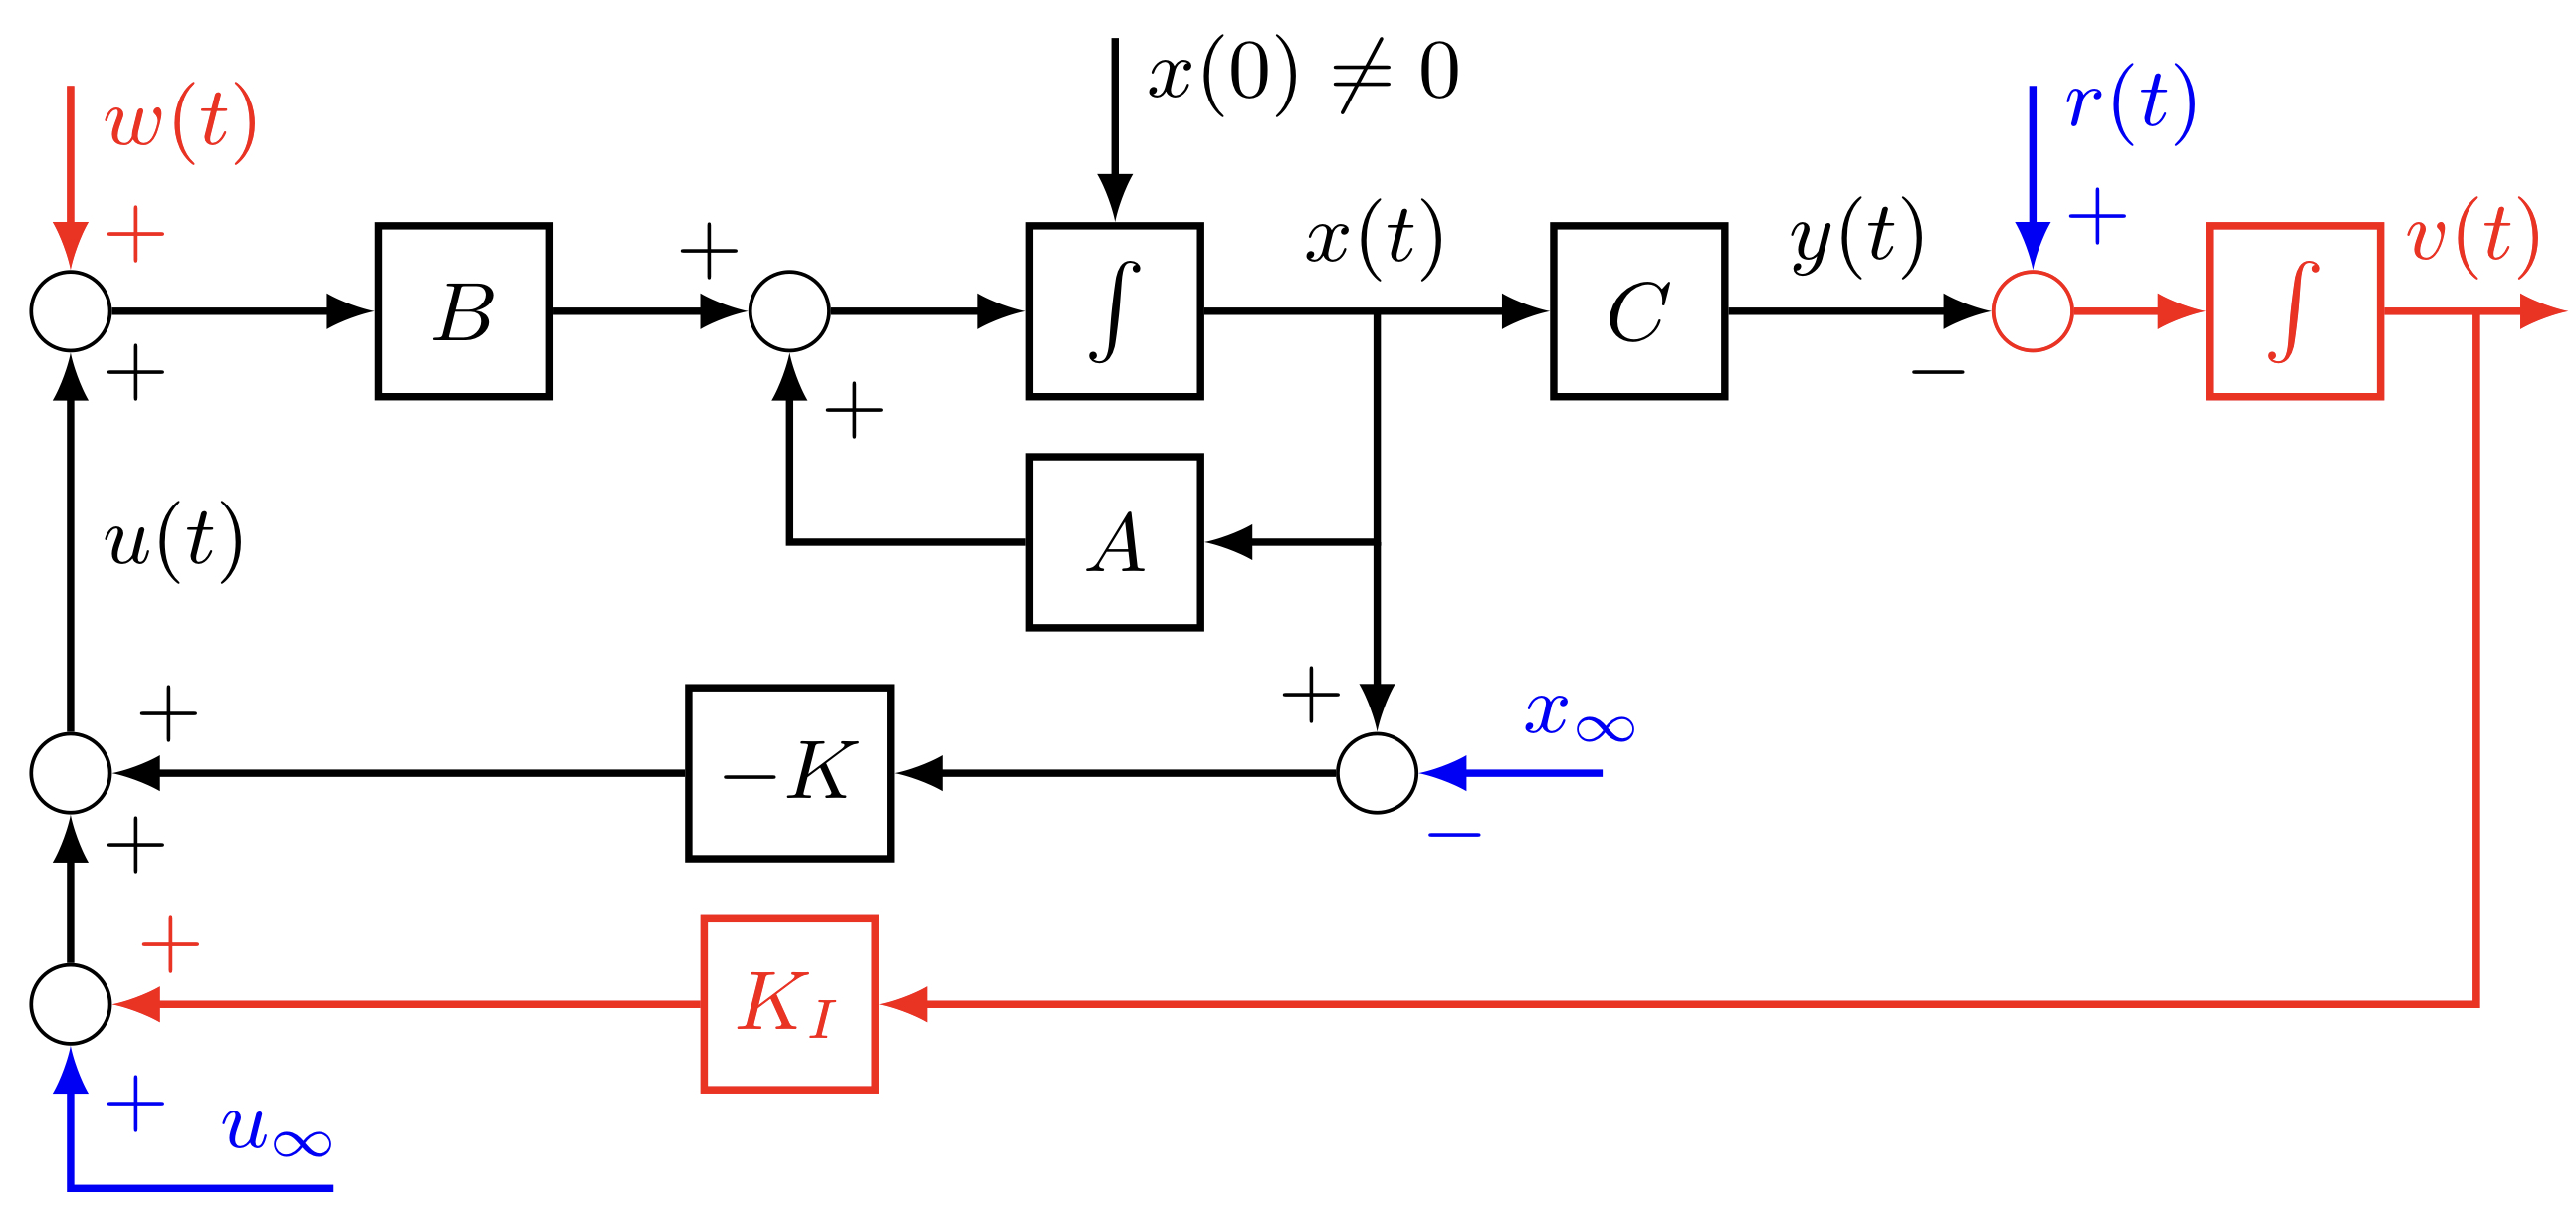
\includegraphics[width = 0.7\linewidth]{images/08/LQR_Folgereg_distreject.jpeg}
    \end{figure}
    Dieser Regler würde auch ohne Feedforward Teil $\{u_\infty(r(t)), x_\infty(r(t))\}$ funktionieren, wäre aber deutlich langsamer.

